\documentclass[
	12pt,				% tamanho da fonte
	openright,			% capítulos começam em pág ímpar (insere página vazia caso preciso)
	oneside,			% para impressão em recto e verso. Oposto a oneside
	a4paper,			% tamanho do papel. 
	english,			% idioma adicional para hifenização
	french,				% idioma adicional para hifenização
	spanish,			% idioma adicional para hifenização
	brazil				% o último idioma é o principal do documento
	]{abntex2}

\usepackage{lmodern}			% Usa a fonte Latin Modern			
\usepackage[T1]{fontenc}		% Selecao de codigos de fonte.
\usepackage[utf8]{inputenc}		% Codificacao do documento (conversão automática dos acentos)
\usepackage{indentfirst}		% Indenta o primeiro parágrafo de cada seção.
\usepackage{color}				% Controle das cores
\usepackage{graphicx}			% Inclusão de gráficos
\usepackage{microtype} 			% para melhorias de justificação
\usepackage{transparent}
\usepackage{eso-pic}
\usepackage{amsthm,amsfonts}
\usepackage{float}
\usepackage{multirow}
\usepackage[table,xcdraw]{xcolor}
\usepackage{lipsum}				% para geração de dummy text
\usepackage[brazilian,hyperpageref]{backref}	 % Paginas com as citações na bibl
\usepackage[alf]{abntex2cite}	% Citações padrão ABNT
\usepackage{xcolor}
\definecolor{verde}{rgb}{0,0.5,0}
\usepackage{listings}
\lstset{
  language=C++,
  basicstyle=\ttfamily\small,
  keywordstyle=\color{blue},
  stringstyle=\color{verde},
  commentstyle=\color{red},
  extendedchars=true,
  showspaces=false,
  showstringspaces=false,
  numbers=left,
  numberstyle=\tiny,
  breaklines=true,
  backgroundcolor=\color{green!10},
  breakautoindent=true,
  captionpos=b,
  xleftmargin=0pt,
}


\titulo{Modelagem Matemática, Simulação e Otimização de Processos}
\autor{Gabriel R. Munhoz 106802\\João Vítor Batistão 108074}
\local{Maringá, PR}
\data{27.11.2021}
\orientador{}
\coorientador{}
\instituicao{%
  Universidade Estadual de Maringá - UEM
  \par
  Departamento de Engenharia de Produção - DEP}
\tipotrabalho{Tese (Doutorado)}
\preambulo{}

\definecolor{blue}{RGB}{41,5,195}

\makeatletter
\hypersetup{
     	%pagebackref=true,
		pdftitle={\@title}, 
		pdfauthor={\@author},
    	pdfsubject={\imprimirpreambulo},
	    pdfcreator={LaTeX with abnTeX2},
		pdfkeywords={abnt}{latex}{abntex}{abntex2}{trabalho acadêmico}, 
		colorlinks=true,       		% false: boxed links; true: colored links
    	linkcolor=blue,          	% color of internal links
    	citecolor=blue,        		% color of links to bibliography
    	filecolor=magenta,      		% color of file links
		urlcolor=blue,
		bookmarksdepth=4
}

\setlength{\parindent}{1.3cm}

\setlength{\parskip}{0.2cm}  % tente também \onelineskip

\makeindex

\usepackage{fancyhdr}
\fancyhead{}
\fancyfoot{}
\lhead{Modelagem Matemática, Simulação e Otimização de Processos}
\rhead{\thepage}

\AddToShipoutPicture{
\put(0,0){
\parbox[b][\paperheight]{\paperwidth}{%
\vfill
\centering
{\transparent{0.1}\includegraphics[scale=1.4]{../../University/Pictures/logoUEM.jpg}    }%
\vfill}}}

%\graphicspath{{../Pictures}}
\begin{document}

\begin{minipage}[c][0cm][c]{0cm} % a primeira minipágina tem uma altura de 1.5cm e uma largura de 3cm.

\centering


\includegraphics[scale=0.45]{../../University/Pictures/uem-modelo-04.png} 
\end{minipage}

\selectlanguage{brazil}

\frenchspacing 

% \pretextual

\imprimircapa


% ---
% RESUMOS
% ---

%\setlength{\absparsep}{18pt} % ajusta o espaçamento dos parágrafos do resumo
%\begin{resumo}
 
 
% \textbf{Palavras-chave}: latex. abntex. editoração de texto.
%\end{resumo}


% ---
% inserir o sumario
% ---
\pdfbookmark[0]{\contentsname}{toc}
\tableofcontents*
\cleardoublepage

% ----------------------------------------------------------
% ELEMENTOS TEXTUAIS
% ----------------------------------------------------------
\textual

\chapter{Introdução}
\pagestyle{fancy}

Este trabalho tem como foco um estudo de caso, que foi pautado em alguns processos estudados, são eles:
Modelagem matemática, Simulação, Otimização e Controle de processos. Esses processos foram utilizados para melhor entendimento do funcionamento de um tanque de agitação que realiza a mistura de água com uma solução aquosa de hidróxido de sódio. 

Para o desenvolvimento desse estudo, é de extrema importância entender minimamente o processo que será modelado, para que assim seja possível uma implementação prática que resulte em um resultado efetivamente assertivo e o mais próximo do real possível. Caso não exista o entendimento do tema proposto, a realização da modelagem matemática, da simulação do processo e por consequência a análise dos dados e a obtenção de otimizações fica totalmente imprecisa. 

\section{Modelagem, simulação e otimização}

A modelagem em conjunto com a simulação e otimização de processos é uma área 

\subsection{Modelagem matemática}

É o montante de relações matemáticas que auxiliam a determinar e descrever o sistema.	Tal modelagem tem objetivos como Melhorar o entendimento do processo, selecionar e treinar os colaboradores da operação, otimizar condições operacionais, dentre outros. \cite{souza2020modelagem}

Existe um processo para a criação desse modelo, primeiro é necessário definir a finalidade do modelo, após isso o processo é descrito através de fluxogramas, então são definidas as considerações e hipóteses simplificadas.
Para a construção do modelo é necessário entender os princípios de conservação e balanços:

Balanço de massa total:
\begin{itemize}
\item Balanço de massa do componente i
\item Balanço de mols total
\item Balanço molar do componente i
\end{itemize}

Tudo isso juntamente com a 1 lei da termodinâmica, com o balanço de energia total, no qual há 3 formas de transferência de energia:

\begin{itemize}
\item Calor(Q): Energia que é transferida através da superfície devido a uma diferença de temperatura.
\item Trabalho: Energia que é transferida através da superfície devido a uma força motriz que não diferença de temperatura (W)
\item Energia advectiva: Energia que se associa a uma corrente de matéria.
\end{itemize}

\subsection{Simulação} 

A simulação dos processos é feita a partir de softwares, um dos softwares que pode ser utilizado é o EMSO. Primeiramente é realizado um fluxograma base para a programação que será implementada posteriormente no software. \cite{souza2020modelagem}

Essa etapa é mais facilmente explicada por meio de um exemplo, é possível analisar esse fluxogramana na Figura \ref{Modelo de exemplo}.

\begin{figure}[H]
\centering
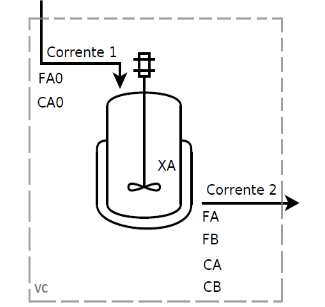
\includegraphics[scale=0.5]{exemplo.png} 
\caption{Modelo de exemplo}
\label{Modelo de exemplo}
\end{figure}

A Imagem \ref{Código EMSO} é um exemplo de como é realizada uma simulação a partir da modelagem do fluxograma anterior no software EMSO.

\begin{figure}[H]
\centering
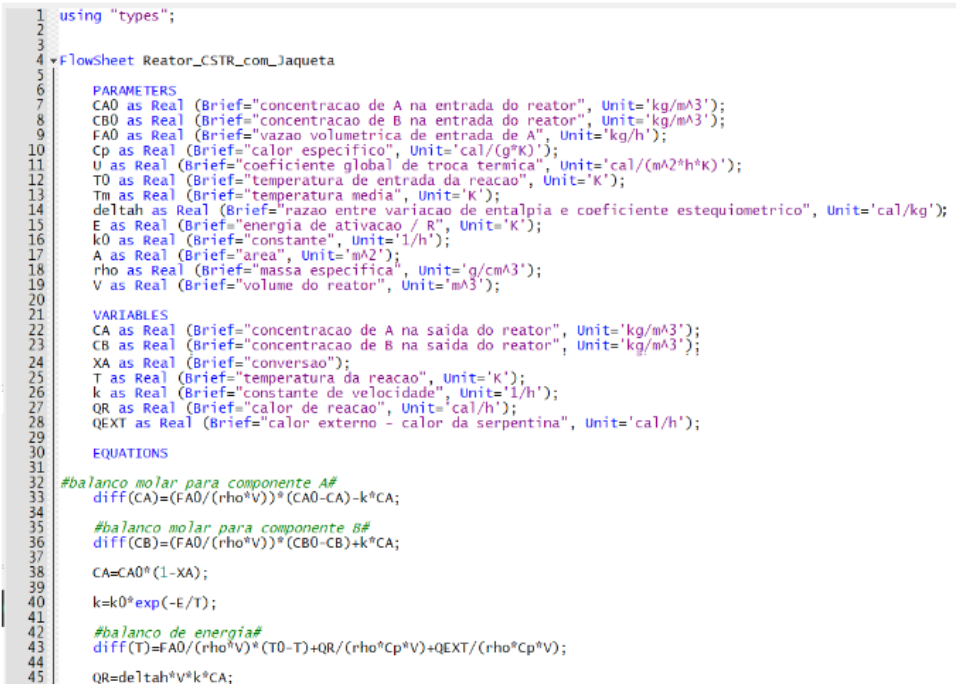
\includegraphics[scale=0.4]{exemplocodigo.png} 
\caption{Código do software EMSO}
\label{Código EMSO}
\end{figure}

Posteriormente a simulação feita no exemplo anterior, é possível geral alguns resultados e consequentemente realizar análises das hipóteses antes levantadas, já que é esse o objetivo da criação e operacionalização do modelo, a seguir é possível verificar gráficos de algumas análises feitas.

\begin{figure}[H]
\centering
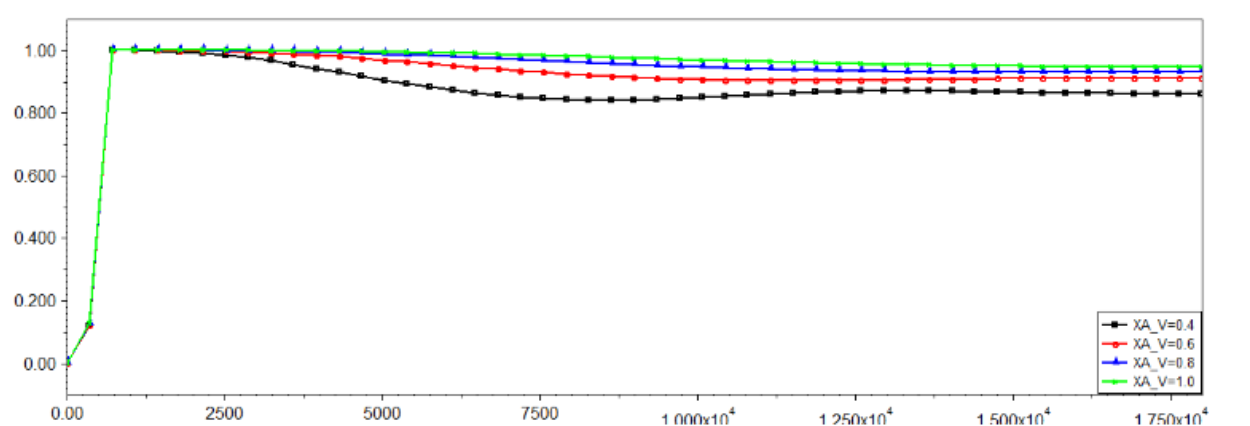
\includegraphics[scale=0.3]{exemplo1.png} 
\caption{Xa em função do tempo}
\label{Modelo de exemplo 1}
\end{figure}

\begin{figure}[H]
\centering
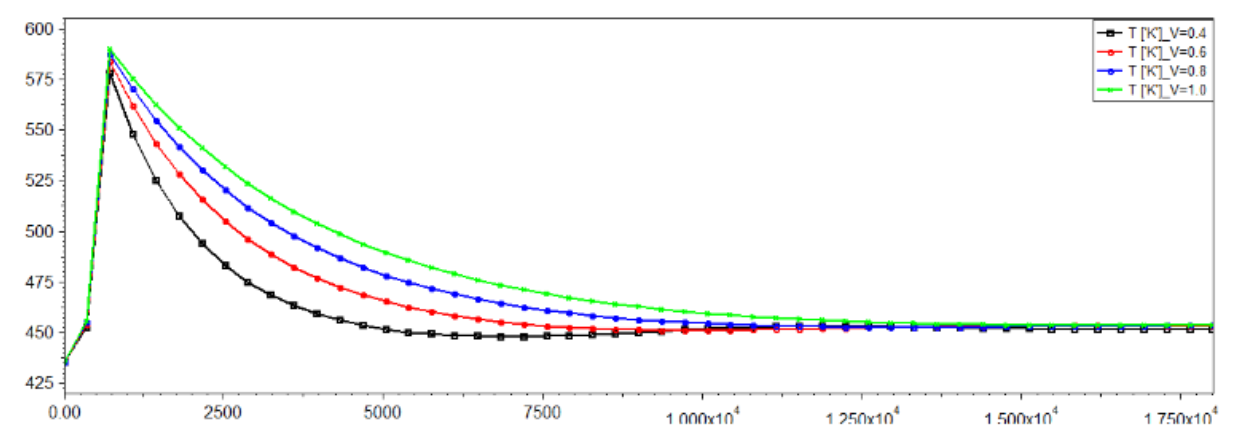
\includegraphics[scale=0.3]{exemplo2.png} 
\caption{Temperatura em relação ao tempo}
\label{Modelo de exemplo 2}
\end{figure}


\subsection{Otimização}

Otimização é a determinação de uma solução rentável e eficiente ou a mais rentável e eficiente a partir de métodos específicos para um problema processual.

Existem vários tipos de otimização na literatura, bem como: Otimizações econômicas que são representadas principalmente pela maximização de lucros, minimização de custos e de investimentos na operação, já as otimizações operacionais são representadas principalmente pela maximização da produção, minimização de consumo de insumos e do delta entre valores desejados e obtidos. 
	
Quanto as aplicações, podemos focar em encontrar um melhor local para a construção de uma planta, encontrar o melhor Layout, minimizar custos de produção, auxílio na alocação de recursos, dentre outros.
	
Uma vez definido o objetivo principal da otimização, passamos a nos preocupar com a formulação do problema de otimização, o qual temos que determinar alguns parâmetros, tais como:
	
\begin{itemize}
\item Função objetivo: Função que representa o problema escolhido para a otimização.
\item Variáveis de decisão: Variáveis que fazem parte da função Objetivo.
\item Restrições: A partir das condições físicas impostas, os limites ao sistema.
\item Região viável: O qual é determinada pelas restrições.
\end{itemize}

Após essa delimitação, chegou o momento da solução do problema, que requer a escolha do método, a análise do processo o estabelecimento dos parâmetros acima citados, aplicação das técnicas matemáticas e a obtenção do resutado.

\subsection{Controle de processos}

Uma vez feito tudo que foi delimitado até o momento, se faz necessário controlar esse processo que já foi otimizado. Par isso é importante a construção do diagrama de controle de processos, o diagrama de blocos, Diagrama P$\&$ID (Diagrama de tubulação e instrumentação).

Ainda assim, existem as estratégias de controle, tais como: Controle feedback, Controle feedfoward,  Controle feedback/feedfoward.

\section{Revisão de Literatura}

Foram selecionaods os seguintes artigos para revisão: 

\begin{enumerate}
\item MODELAGEM E SIMULAÇÃO DE UM REATOR DO TIPO CSTR NÃO ISOTÉRMICO NO SOFTWARE EMSO \cite{souza2020modelagem}
\item SIMULAÇÃO DO REATOR QUÍMICO DE RETROMISTURA NO SOFTWARE EMSO \cite{schultz2013simulaccao}
\end{enumerate}

O primeiro se trata de um modelo matemático de um reator CSTR através do software EMSO, com o objetivo de otimizar a qualidade dos processos, entender os fenômenos e mitigar os custos referentes a produção propriamente dita. Segundo o artigo estudado, o reator CSTR tem como características principais a presença de mistura perfeita no meio, com ausência de variações dos estados e nesse contexto o artigo demonstra a modelagem de tal reator, envolvendo balanços de energia, além da simulação de vários cenários com o fim de compreender de forma mais profunda a eficiência da produção em uma indústria química.

Já no segundo artigo explicitado, tem um foco maior na otimização de processos que proporciona melhorias nas especificações dos produtos, redução de custos também em reatores químicos, mas agora com um foco maior na parte de desenvolvimento de melhorias, redução de custos e otimizações no geram a partir da criação do modelo matemático, e com o foco maior na análise que essa modelagem e simulação trás.
	
Ambos os artigos utilizam o software EMSO por sem um software de alto desempenho, capaz de realizar simulações em equipamentos ou processos que tenham sido modelados de antemão.

\section{Objetivos e contribuições}

O presente trabalho possui como objetivo a modelagem, simulação e otimização de um processo de mistura que ocorre em tanque de agitação. Esses processos serão realizados no software EMSO. Esse estudo é de extrema importância para auxiliar a tomada de decisão por meio do uso de software de simulação e otimização. 

Por meio desse trabalho prático de modelagem matemática no software EMSO será possível verificar como é realiza uma análise em conjunto com resultados advindos de uma simulação. Assim como a verificação de possíveis incongruências e dados não consistentes.

\newpage
\chapter{Modelagem Matemática}
\pagestyle{fancy}

O sistema que será estudado é um tanque agitado com duas correntes de entrada, uma sendo água pura e a outra uma solução aquosa de hidróxido de sódio. Há também uma corrente de saída, um agitador e um controlador conforme a Figura \ref{Modelo do Tanque} que retrata o modelo que será simulado.

\begin{figure}[!h]
\centering
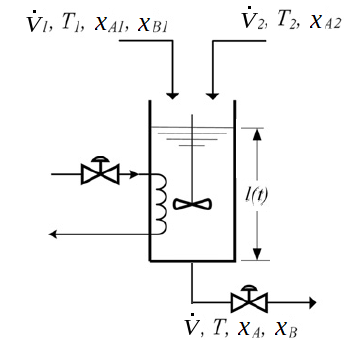
\includegraphics[scale=0.6]{1a.png} 
\caption{Modelo do Tanque}
\label{Modelo do Tanque}
\end{figure}

Para realizar a modelagem desse tanque é necessário estabelecer certas hipóteses para tornar os cálculos mais simples e capazes de serem simulados. As hipóteses que foram estabelecidos são:

\begin{itemize}
\item Mistura perfeita;
\item Propriedades físicas constantes;
\item Calor de mistura desprezível;
\item Tanque isolado e $\dot{W}_{s}$ é desprezível.
\end{itemize}

A primeira equação que é possível derivar das informações do modelo é o balanço de massa global. Em que é definido um equilíbrio de massa, tudo que entra no sistema é equivalente ao que sai. 

\begin{equation}
\frac{d(\rho V)}{dt}=\sum\limits_{i=1}^{n}\dot{V}_{e,i}-\rho_{e,i}-\sum\limits_{j=1}^{m}\dot{V}_{s,j}-\rho_{s,j}
\end{equation}

Sabendo-se que n = 2 e m = 1, pois existem 2 correntes de entrada e apenas 1 de saída tem-se: 

\begin{equation}
\frac{d(\rho V)}{dt}=(\rho_{1}\dot{V}_{1}+\rho_{2}\dot{V}_{2})-\rho \dot{V}
\end{equation}

Devido a consideração de que as propriedades físicas são constantes em qualquer ponto do tanque as densidades são iguais e podem ser retiradas do balanço de massa global.

\begin{equation}
\rho=\rho_{1}=\rho_{2}
\end{equation}

\begin{equation}
\frac{dV}{dt}=(\dot{V}_{1}+\dot{V}_{2})-\dot{V}
\end{equation}

Sendo o volume é V = A.l, é possível chegar na equação 2.5.

\begin{equation}
A\frac{dl}{dt}=\dot{V}_{1}+\dot{V}_{2}-\dot{V}
\end{equation}

E a partir dessa pode-se isolar a derivada $\frac{dl}{dt}$ para chegar na seguinte equação:

\begin{equation}
\frac{dl}{dt}=\frac{(\dot{V}_{1}+\dot{V}_{2}-\dot{V})}{A}
\end{equation}

E outras equações que são possíveis de derivar do modelo são os balanços de massa por componente. Para o componente A:

\begin{equation}
\frac{d(x_{A}V)}{dt}=(x_{A,1}\dot{V}_{1}+x_{A,2}\dot{V}_{2})-x_{A}\dot{V}
\end{equation}

Realizando a regra do produto na equação 2.7, tem-se:

\begin{equation}
V\frac{dx_{A}}{dt}+x_{A}\frac{dV}{dt}=(x_{A,1}\dot{V}_{1}+x_{A,2}\dot{V}_{2})-x_{A}\dot{V}
\end{equation}

Substituindo a equação 2.6 na equação anterior, tem-se:

\begin{equation}
V\frac{dx_{A}}{dt}+x_{A}(\dot{V}_{1}+\dot{V}_{2}-\dot{V})=(x_{A,1}\dot{V}_{1}+x_{A,2}\dot{V}_{2})-x_{A}\dot{V}
\end{equation}

\begin{equation}
V\frac{dx_{A}}{dt}=\dot{V}_{1}(x_{A,1}-x_{A})+\dot{V}_{2}(x_{A,2}-x_{A})
\end{equation}

\begin{equation}
Al\frac{dx_{A}}{dt}=\dot{V}_{1}(x_{A,1}-x_{A})+\dot{V}_{2}(x_{A,2}-x_{A})
\end{equation}

De forma similar é realizado para o componente B:

\begin{equation}
\frac{d(x_{B}V)}{dt}=(x_{B,1}\dot{V}_{1}+x_{B,2}\dot{V}_{2})-x_{B}\dot{V}
\end{equation}

Realizando a regra do produto na equação 2.12, tem-se:

\begin{equation}
V\frac{dx_{B}}{dt}+x_{B}\frac{dV}{dt}=(x_{B,1}\dot{V}_{1}+x_{B,2}\dot{V}_{2})-x_{B}\dot{V}
\end{equation}

Substituindo a equação 2.6 na equação anterior, tem-se:

\begin{equation}
V\frac{dx_{B}}{dt}+x_{B}(\dot{V}_{1}+\dot{V}_{2}-\dot{V})=(x_{B,1}\dot{V}_{1}+x_{B,2}\dot{V}_{2})-x_{B}\dot{V}
\end{equation}

\begin{equation}
V\frac{dx_{B}}{dt}=\dot{V}_{1}(x_{B,1}-x_{B})+\dot{V}_{2}(x_{B,2}-x_{B})
\end{equation}

\begin{equation}
Al\frac{dx_{B}}{dt}=\dot{V}_{1}(x_{B,1}-x_{B})+\dot{V}_{2}(x_{B,2}-x_{B})
\end{equation}

Por fim, outra equação também pode ser modelada a partir das informações do tanque, e para chegar nela é necessário partir do balanço de energia, que é mostrado na equação abaixo.

\begin{equation}
\frac{dE_{T}}{dt}=\sum\limits_{i=1}^{n}\dot{M}_{i}\overline{E}_{T,i}-\sum\limits_{j=1}^{m}\dot{M}_{j}\overline{E}_{T,j}+\dot{Q}+\dot{W}
\end{equation}

Sabendo que $E_{T}=E_{k}+E_{p}+U$, tem-se:

\begin{equation}
\frac{d(E_{k}+E_{p}+U)}{dt}=\sum\limits_{i=1}^{n}\dot{M}_{i}(\overline{E}_{k,i}+\overline{E}_{p,i}+\overline{U}_{i})-\sum\limits_{j=1}^{m}\dot{M}_{j}(\overline{E}_{k,j}+\overline{E}_{p,j}+\overline{U}_{j})+\dot{Q}+\dot{W}
\end{equation}

No modelo estudado as energias cinética e potencial assim como o trabalho são desprezíveis e igualados a 0. E como o objeto de estudo é líquido pode-se afirmar que $\frac{dU}{dt}\approx\frac{dH}{dt}$. Assim, a equação 2.18 pode ser simplificada para a equação 2.20 por meio da substituição da energia interna por entalpia, equação 2.19.

\begin{equation}
\frac{dU}{dt}\approx\frac{dH}{dt}=\rho C_{p}V\frac{dT}{dt}
\end{equation}

\begin{equation}
\overline{\rho}\overline{C}_{p}Al\frac{dT}{dt}=\overline{\rho}\overline{C}_{p}\dot{V}_{1}(T_{1}-T)+\overline{\rho}\overline{C}_{p}\dot{V}_{2}(T_{2}-T)+\dot{Q}
\end{equation}

Assim, o conjunto das equações 2.5, 2.11, 2.16 e 2.20 que foram encontradas a partir dos balanços de massa, global e de componentes, e o balanço de energia definem o modelo matemático completo do sistema e torna possível realizar a simulação do tanque.

\newpage
\chapter{Simulação Dinâmica}
\pagestyle{fancy}

Para realização da simulação foi escolhido o software EMSO e o código utilizado no software se encontra no Apêndice A. O tanque do sistema foi descrito como cilindrico e com diâmetro de 2,76 m e os outros dados utilizados na simulação foram:

\begin{itemize}
\item Área do tanque (A) = 5,983 $m^{2}$;
\item Calor ($\dot{Q}$) = 100000 kW;
\item Densidade do líquido ($\rho$) = 1000 $kg/m^{3}$;
\item Calor específico do líquido ($C_{p}$) = 4,18 kJ/(kg*K);
\item Temperatura da corrente 1 ($T_{1}$) = 323 K;
\item Temperatura da corrente 2 ($T_{2}$) = 293 K;
\item Composição de água na corrente 1 ($x_{a,1}$) = 0,4;
\item Composição de hidróxido de sódio na corrente 1 ($x_{b,1}$) = 0,6;
\item Composição de água na corrente 2 ($x_{a,2}$) = 1,0;
\item Composição de hidróxido de sódio na corrente 2 ($x_{b,2}$) = 0,0;
\item Vazão de saída do tanque ($\dot{V}$) = 0,3 $\sqrt{l}$ $m^{3}/s$;
\item Vazão de entrada da corrente 1 ($\dot{V}_{1}$) = 0,3 $m^{3}/s$;
\item Vazão de entrada da corrente 2 ($\dot{V}_{2}$) = 0,15 $m^{3}/s$;
\item Tempo de simulação (t) = 100000 s;
\end{itemize}

Condições Iniciais:

\begin{itemize}
\item Temperatura (T) = 293 K;
\item Altura da mistura (l) = 2,0 m;
\item Composição de água ($x_{a}$) = 1,0;
\item Composição de hidróxido de sódio ($x_{b}$) = 0,0;
\end{itemize}

Assim, a partir da simulação dos dados acima foi possível montar a tabela \ref{Resultados da simulação} com os resultados obtidos.

\begin{table}[H]
\centering
\caption{Resultados da simulação}
\label{Resultados da simulação}
\resizebox{\textwidth}{!}{%
\begin{tabular}{c|c|c|c}
\rowcolor[HTML]{EFEFEF} 
Temperatura (T) & Altura da mistura (l) & Composição de água ($x_{a}$) & Composição de hidróxido de sódio ($x_{b}$) \\
366,16 & 2,25 & 0,6 & 0,4
\end{tabular}%
}
\end{table}

Foram gerados gráficos da temperatura, das composições dos componentes e da altura da mistura no tanque pelo tempo, focando nos instantes iniciais (t $\leq$ 300 s) para verificação das variações. A temperatura e a altura da mistura foram aumentando conforme os gráficos \ref{Gráfico da temperatura x tempo} e \ref{Gráfico da altura x tempo}, e as concentrações de água e de hidróxido de sódio também foram variando de acordo com o gráfico \ref{Gráfico da composição dos componentes x tempo}. 

\begin{figure}[H]
\centering
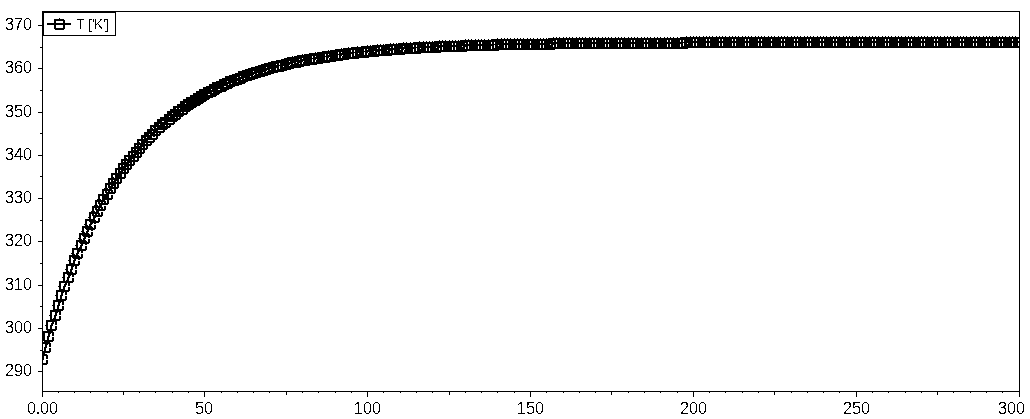
\includegraphics[scale=0.4]{Plot2D (7).png} 
\caption{Gráfico da temperatura (T) x tempo (t)}
\label{Gráfico da temperatura x tempo}
\end{figure}

\begin{figure}[H]
\centering
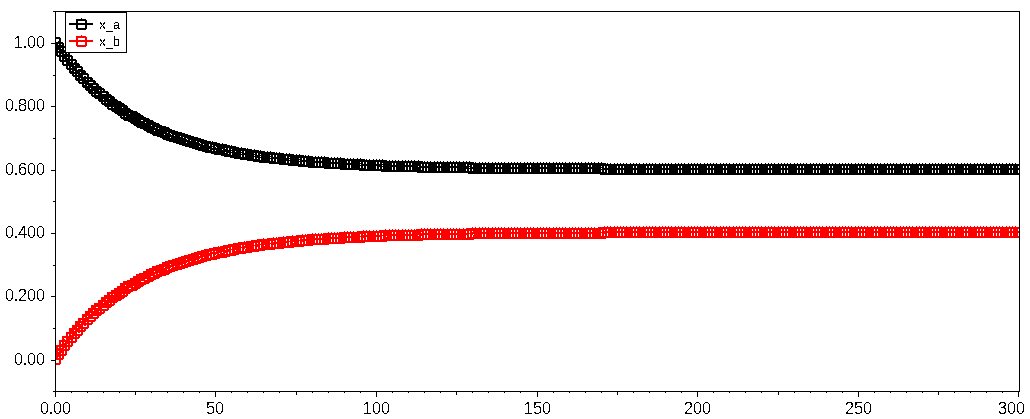
\includegraphics[scale=0.4]{Plot2D (6).png} 
\caption{Gráfico da composição de água e de hidróxido de sódio ($x_{a}$ e $x_{b}$) x tempo (t)}
\label{Gráfico da composição dos componentes x tempo}
\end{figure}

\begin{figure}[H]
\centering
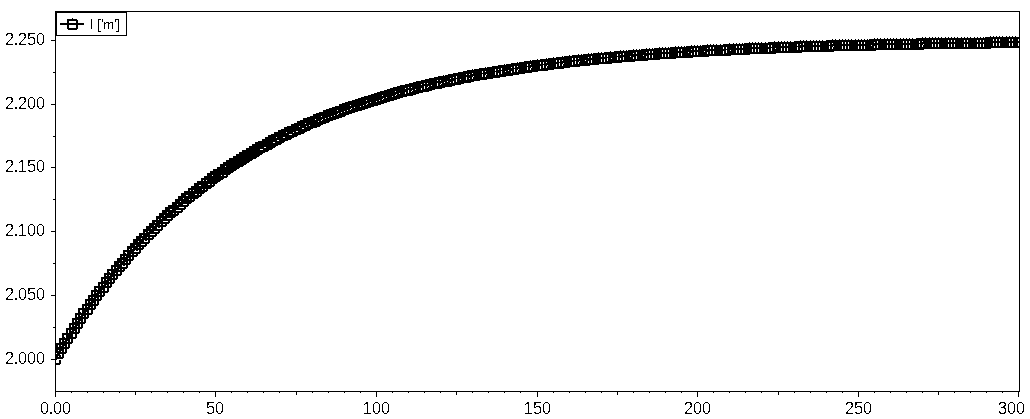
\includegraphics[scale=0.4]{Plot2D (8).png} 
\caption{Gráfico da altura da mistura no tanque (l) x tempo (t)}
\label{Gráfico da altura x tempo}
\end{figure}

A partir desses resultados é possível notar que a temperatura aumenta de forma rápida no sistema e entra em equilíbrio próximo de 150 segundos. O aumento da temperatura de 293 K para 366,16 K é possivelmente derivado da entrada da corrente 1 a 323 K em conjunto com a tranformação da energia interna da mistura em energia térmica.

As composições de água e de hidróxido de sódio também se equilibram próximo de 150 segundos. A concentração de água diminui no tanque de 100$\%$ para 60$\%$ e a concentração de hidróxido de sódio aumenta de 0$\%$ para 40$\%$, isso ocorre devido a maior vazão da corrente 1 que possui uma concentração maior de hidróxido de sódio e menor de água. 

Portanto, no tanque ocorre uma diluição da solução aquosa de hidróxido de sódio que entra pela corrente 1, diminuindo a concentração desse componente de 60$\%$ para 40$\%$. Contudo, devido a agitação a mistura acaba sendo aquecida para 366,16 K e a mistura chega a uma altura de 2,25 m.

\newpage
\chapter{Otimização Estacionária}
\pagestyle{fancy}

A otmização proposta neste trabalho foi a de maximizar a concentração de hidróxido de sódio na corrente de saída, sendo assim a função objetiva se resume ao valor de $x_{b}$. Para realizar uma otimização é necessário estabelecer restrições para o sistema, e as restrições utilizadas nesse modelo foram:

\begin{eqnarray}
1 m &\leq l \leq &4 m\\
293 K &\leq T \leq &343 K
\end{eqnarray}

Assim como a simulação, a otimização também foi realizada no software EMSO e o código utilizado está presente no Apêndice A. Para maximizar a concentração de $x_{b}$ foi liberado para o software variar apenas a vazão de entrada da corrente 1. E possivelmente devido isso e as restrições estabelecidas, o software não conseguiu gerar resultados convergentes. 

É possível observar que, durante a simulação do sistema a temperatura da mistura foi elevada a 366,16 K, contudo na otimização do modelo há uma restrição de temperatura máxima para 343 K. Logo, é possível concluir que com as restrições estabelecidas na otimização não é possível melhorar o processo e que talvez nem seja possível a realização da mistura, visto que a temperatura que é atingida na simulação ultrapassa a restrição de temperatura máxima da otimização.


\newpage
\chapter{Simbologia}
\pagestyle{fancy}

\begin{itemize}
\item Q - Calor - Unidade: kJ;
\item $\dot{Q}$ - Taxa de calor - Unidade: kW;
\item $C_{p}$ - Calor específico - Unidade: kJ/(kg*K);
\item $\rho$ - Densidade - Unidade: $kg/m^{3}$;
\item $x$ - Concentração - Unidade: pu;
\item V - Volume - Unidade: $m^{3}$;
\item $\dot{V}$ - Vazão do líquido - Unidade: $m^{3}/s$;
\item A - Área - Unidade: $m^{2}$;
\item l - Altura - Unidade: m;
\item T - Temperatura - Unidade: K;
\item $E_{T}$ - Energia total - Unidade: kJ;
\item $E_{p}$ - Energia potencial - Unidade: kJ;
\item $E_{k}$ - Energia cinética - Unidade: kJ;
\item U - Energia interna - Unidade: kJ;
\item H - Entalpia - Unidade: kJ/mol;
\item m - Massa - Unidade: kg;
\item $\dot{M}$ - Vazão mássica - Unidade: kg/s;
\end{itemize}

\newpage
\postextual

\bibliography{referencia}

\begin{anexosenv}

\chapter{Código utilizado no software EMSO}

\begin{lstlisting}
using "types";
 
Model Tanque

	PARAMETERS
	A 			as area;
	Q 			as heat_rate;
	Cp 			as cp_mass;
	rho 			as dens_mass;
	
	VARIABLES
	l 			as length;
	x_a1			as fraction;
	x_b1			as fraction;
	T1			as temperature;
	V1			as flow_vol;
	x_a2			as fraction;
	x_b2			as fraction;
	T2			as temperature;
	V2			as flow_vol;
	x_a			as fraction;
	x_b			as fraction;
	T			as temperature;
	V			as flow_vol;
	
	EQUATIONS
	"Balanco de massa global"
	diff(l) * A = V1 + V2 - V;

	"Balanco de massa para componente A"
	diff(x_a) * A * l = V1 * (x_a1 - x_a) + V2 * (x_a2 - x_a);
	
	"Balanco de massa para componente B"
	diff(x_b) * A * l = V1 * (x_b1 - x_b) + V2 * (x_b2 - x_b);

	"Balanco de energia para o tanque"
	diff(T) * rho * Cp * A * l = (rho * Cp * V1) * (T1 - T) + (rho * Cp * V2) * (T2 - T) + Q;

end

FlowSheet Avaliacao

	DEVICES
	tanque 		as Tanque;
	
	SET
	tanque.A = 5.983 * 'm^2';
	tanque.Q = 100000 * 'kW';
	tanque.rho = 1000 * 'kg/m^3';
	tanque.Cp = 4.18 * 'kJ/(kg*K)';
	
	SPECIFY
	tanque.T1 = 323 * 'K';
	tanque.T2 = 293 * 'K';
	tanque.x_a1 = 0.4;
	tanque.x_b1 = 0.6;
	tanque.x_a2 = 1.0;
	tanque.x_b2 = 0.0;
	tanque.V = 0.3 * ((tanque.l)^(0.5)) * 'm^3/s';
	# 1080 m^3/h
	tanque.V1 = 0.3 * 'm^3/s';
	# 540 m^3/h
	tanque.V2 = 0.15 * 'm^3/s';
	
	INITIAL
	tanque.T = 293 * 'K';
	tanque.l = 2.0 * 'm';
	tanque.x_a = 1.0;
	tanque.x_b = 0.0;
	
	OPTIONS
	TimeStep = 1;
	TimeEnd = 100000;
	TimeUnit = 's';

end

Optimization OtimizacaoDoXb as Avaliacao
	
	MAXIMIZE
	tanque.x_b;

	FREE
	tanque.V1;	
	
	EQUATIONS
	tanque.l <= 4 * 'm';
	tanque.l >= 1 * 'm';
	tanque.T <= 343 * 'K';
	tanque.T >= 293 * 'K';
	
	OPTIONS
	Dynamic = false;
	
end \end{lstlisting}

\end{anexosenv}

\end{document}
